\documentclass[10pt,twocolumn]{article}

\usepackage[a4paper,top=17mm,bottom=19mm,left=17mm,right=17mm,columnsep=7mm]{geometry}
\usepackage{amsmath}
\usepackage{booktabs}
\usepackage{graphicx}
\usepackage{microtype}
\usepackage{tabularx}
\usepackage{enumitem}
\usepackage{xcolor}
\usepackage[numbers,sort&compress]{natbib}
\usepackage[hidelinks]{hyperref}
\usepackage{fancyhdr}
\usepackage{balance}
\usepackage{tikz}
\usepackage{pgfplots}
\pgfplotsset{compat=1.18}
\usetikzlibrary{arrows.meta,positioning}

\definecolor{btlblue}{HTML}{172B4D}
\definecolor{btlrule}{HTML}{B9C2CF}
\definecolor{btlshade}{HTML}{F3F5F8}
\definecolor{btlgreen}{HTML}{197D6D}
\definecolor{btlamber}{HTML}{CC742E}

\setlength{\parindent}{1em}
\setlength{\parskip}{0pt}
\setlist{nosep,leftmargin=*}
\renewcommand{\arraystretch}{1.08}
\hypersetup{colorlinks=true,linkcolor=btlblue,urlcolor=btlgreen,citecolor=btlblue}

\pagestyle{fancy}
\fancyhf{}
\fancyhead[L]{\footnotesize BAD THEORY LABS}
\fancyhead[R]{\footnotesize Interference Search}
\fancyfoot[C]{\footnotesize\thepage}
\renewcommand{\headrulewidth}{0.3pt}

\newcommand{\code}[1]{\texttt{#1}}
\newcommand{\IS}{Interference Search}

\begin{document}

\twocolumn[
\begin{center}
{\LARGE\bfseries\color{btlblue} Interference Search}\par
\vspace{2mm}
{\large Reasoning over merged states, many branches at once}\par
\vspace{4mm}
{\normalsize Al-ameen, Bad Theory Labs}\par
{\small Lagos, September 2026}\par
\end{center}

\begin{minipage}{0.90\textwidth}
\small
\textbf{Abstract.}
Language models reason in a line: one token after another in a single transcript, rewinding in text when a step fails. I study a different shape. \IS{} works on explicit states. Every live branch expands at once, the environment executes the moves, branches that reach the same state merge, a small trained judge cancels dead ends, and the survivors advance together one level at a time. The name comes from the way quantum search lets wrong paths cancel; the method is classical and claims no quantum speedup. On 30 hard Countdown problems, with the same judge and the same budget of 200 judged positions, \IS{} solves 30 and a single line of thought solves 21; to solve all 30, the line needs 23.7 sequential steps on average and the frontier needs 3. Most reasoning in this domain is duplicate work: at six numbers, 831,176 operation sequences collapse into 13,229 distinct states. The judge, trained on four- and five-number problems, cut the search 12.6 times on seven-number problems without losing a solution, but loses solutions on hard problems when set aggressively. Qwen3-1.7B thinking in text solves 3 of the 30 problems; in one recorded trace it wrote the correct expression at token 1,313 and never committed to it. On 30 MBPP problems the model fails on its first try, \IS{} solves 9 against 8 for independent sampling and 7 for both linear refinement strategies, a lead within noise. Several obvious alternatives failed, and I report them: textual notes about failed attempts made the model retry them, decode-time rewinding regenerated the same mistake, and parallel streams that could attend to each other learned nothing that independent streams did not. None of these results trains the language model; that is the next step.
\end{minipage}
\vspace{6mm}
]

\section{The problem with a line}

A reasoning model today holds one line of thought. It can explore alternatives only by writing them out in sequence, and the alternatives it has dropped stay buried in the transcript. Running several copies in parallel does not fix this: independent samples from one model share its biases, so they tend to fail in the same way. In my Countdown runs with Qwen3-1.7B \citep{qwen3}, 45.1\% of failed attempts repeated an attempt the same sample had already rejected, and a further 29.7\% repeated one that a sibling sample had rejected earlier.

The clearest case is a single trace. Given $[24, 98, 19, 3]$ and the target 361, the model wrote $((24 \times 19) - 98) + 3 = 361$ at token 1,313. It checked the expression nine more times, drifted back into wrong combinations, and reached its 2,048-token budget without giving an answer. The knowledge was present. The format could not hold it, compare it against alternatives, or commit to it.

Quantum search offers a picture of the alternative. Grover's algorithm \citep{grover1996} applies one check to a superposition of every candidate and uses the sign of the amplitudes so that wrong candidates fade together. A classical machine cannot reproduce the speedup, and I do not claim one. Two parts of the picture do survive classically. Many paths collapse into far fewer states when the problem has structure, so a reasoner that works on states handles many paths at the cost of one state each. And one refutation of a state removes every path through it, including paths that were never written out.

\paragraph{Contributions.}
\begin{itemize}
\item \IS{}, a search loop over explicit states with merging, a learned judge and a level-synchronous frontier, applied to both thinking (proposing and judging) and execution (applying moves, running tests) (\S\ref{sec:method}).
\item Exact measurements of how much of Countdown's search space is duplicate or dead, and a judge that generalizes to larger problems than it was trained on (\S\ref{sec:redundancy}, \S\ref{sec:judge}).
\item Matched-compute comparisons and ablations showing that the gain comes from merging plus level-synchronous advance, and that neither a global ranked memory nor plain cross-stream attention reproduces it (\S\ref{sec:shape}).
\item Results with a real language model and in code, and a set of negative results that constrain where the mechanism has to live (\S\ref{sec:llm}, \S\ref{sec:code}).
\end{itemize}

\begin{figure}[t]
\centering
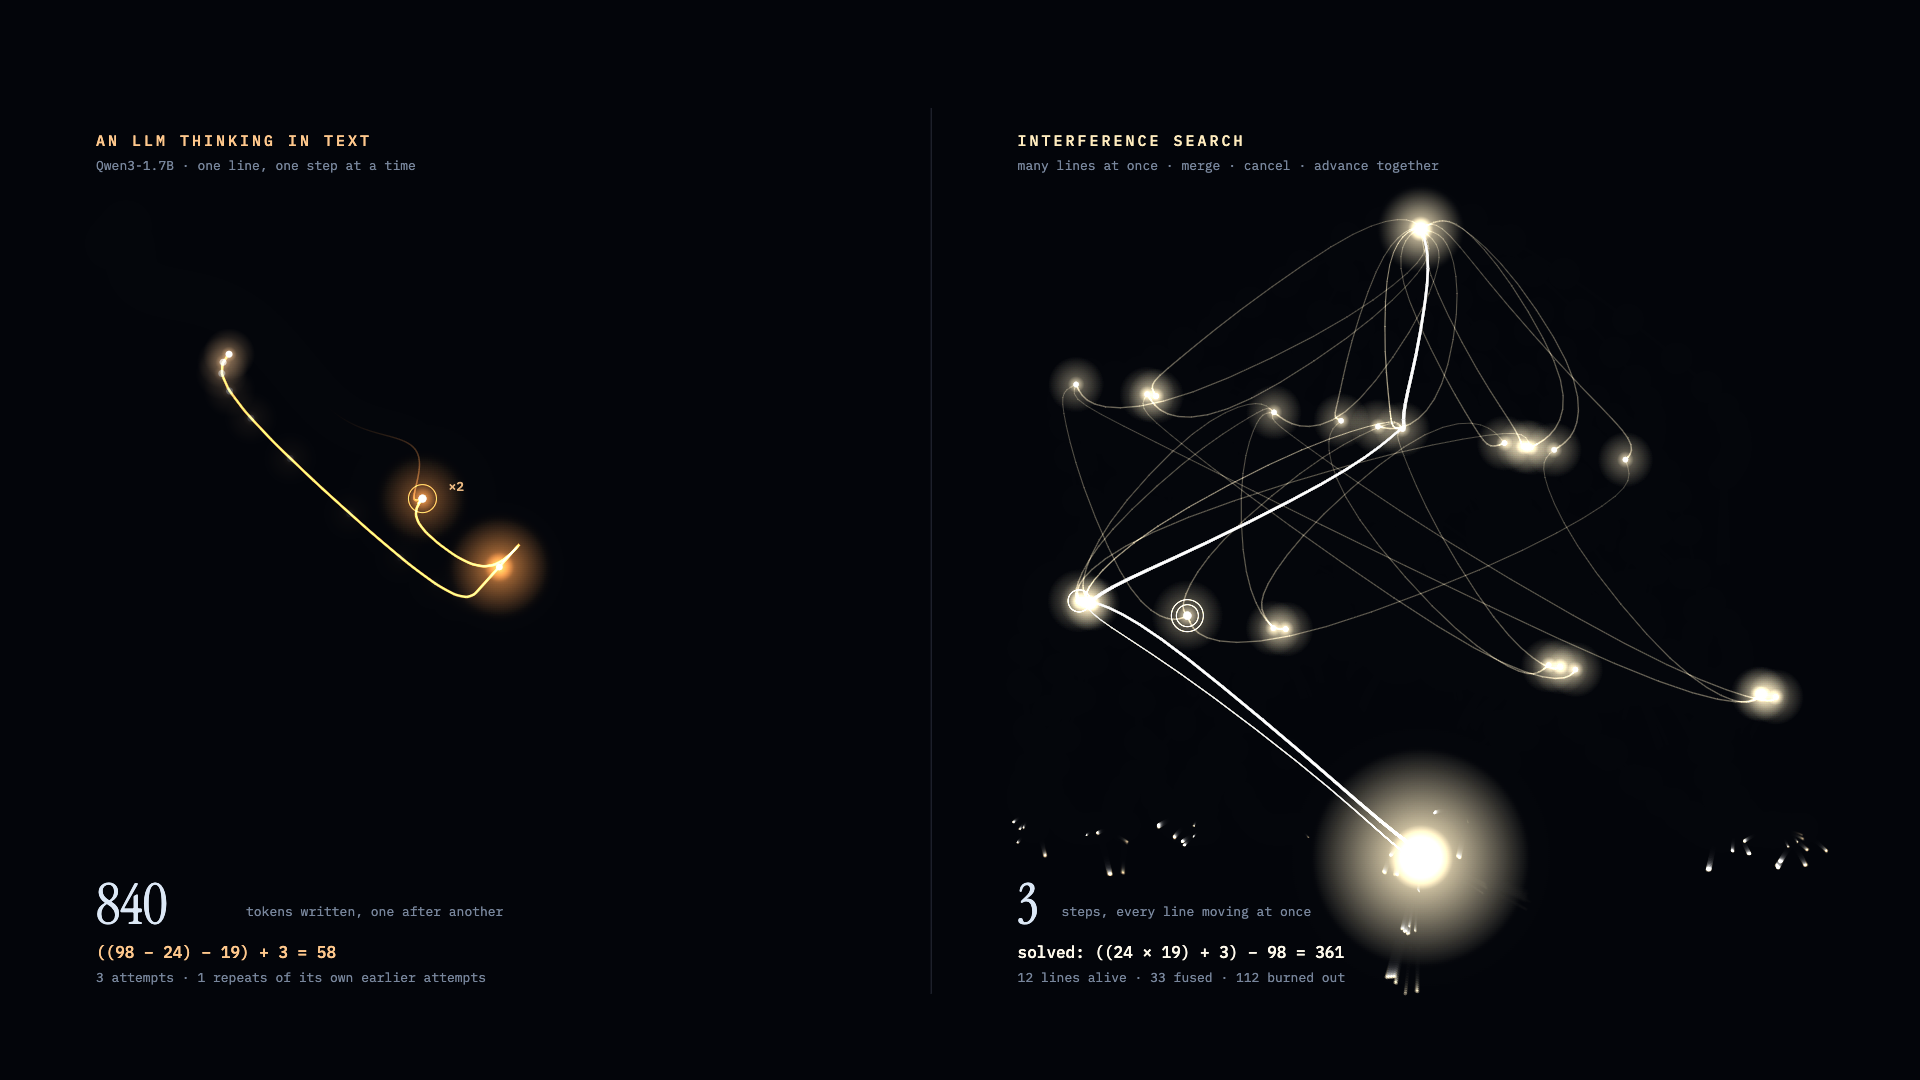
\includegraphics[width=\columnwidth]{figures/teaser.png}
\caption{The same problem solved two ways. Left: Qwen3-1.7B's recorded reasoning, with every attempt placed where it was written; the rings mark repeats. Right: \IS{} expanding many branches, fusing duplicates, burning out dead ends and reaching $((24 \times 19) + 3) - 98 = 361$ in three steps.}
\label{fig:teaser}
\end{figure}

\section{Interference Search}
\label{sec:method}

A domain supplies five functions: a start state, a proposer that returns candidate next states for each live state, a merge key that says when two states are the same situation, a judge that scores states, and goal and dead-end tests. Cost is counted in the domain's own unit: judged states in Countdown, generated tokens in code.

\begin{figure}[t]
\centering
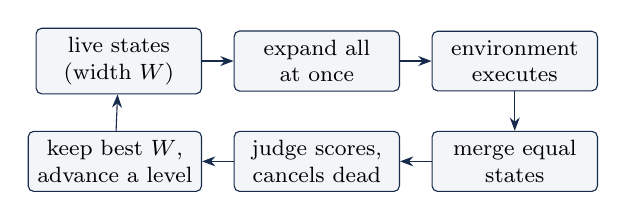
\begin{tikzpicture}[node distance=5mm and 4mm, every node/.style={font=\footnotesize}, box/.style={draw=btlblue, rounded corners=2pt, fill=btlshade, minimum width=21mm, minimum height=6mm, align=center}]
\node[box] (live) {live states\\(width $W$)};
\node[box, right=of live] (exp) {expand all\\at once};
\node[box, right=of exp] (exe) {environment\\executes};
\node[box, below=of exe] (merge) {merge equal\\states};
\node[box, left=of merge] (judge) {judge scores,\\cancels dead};
\node[box, left=of judge] (keep) {keep best $W$,\\advance a level};
\draw[-{Stealth}, btlblue] (live) -- (exp);
\draw[-{Stealth}, btlblue] (exp) -- (exe);
\draw[-{Stealth}, btlblue] (exe) -- (merge);
\draw[-{Stealth}, btlblue] (merge) -- (judge);
\draw[-{Stealth}, btlblue] (judge) -- (keep);
\draw[-{Stealth}, btlblue] (keep) -- (live);
\end{tikzpicture}
\caption{One round of \IS{}. Nothing carries between rounds except the states and a memory of merge keys already expanded.}
\label{fig:loop}
\end{figure}

Each round (Figure~\ref{fig:loop}) expands every live state, executes the proposed moves, and pools the resulting states by merge key. A state that several parents reach is kept once; the ranks at which parents proposed it are pooled as votes. States whose keys were already expanded are dropped, which is the memory that stops a branch from revisiting its own failures. The judge scores the pool, the best $W$ survive, and all survivors move to the next level together. The width $W$ is chosen from the budget, so a larger budget buys a wider frontier rather than a longer chain. The loop never carries a transcript; each proposal sees one state.

The baseline for every comparison uses the same five functions in a single chain: judge the children of the current state, sample one in proportion to its score, continue, and restart from the beginning when the chain dies.

\section{Where the redundancy is}
\label{sec:redundancy}

Countdown makes the structure exact. A state is the sorted multiset of available numbers; a move combines two of them with $+$, $-$, $\times$ or $\div$, with positive whole results; the goal is a single number equal to the target. Dynamic programming over states labels every state as alive or dead.

\begin{table}[t]
\centering\small
\begin{tabular}{lrrrr}
\toprule
Numbers & Paths & States & Paths/state & Dead share \\
\midrule
4 & 566 & 159 & 3.6$\times$ & 95.4\% \\
5 & 17,266 & 1,511 & 11.4$\times$ & 96.2\% \\
6 & 831,176 & 13,229 & 62.8$\times$ & 82.6\% \\
\bottomrule
\end{tabular}
\caption{Path compression at the deepest non-terminal level, mean over 20 random solvable instances per size. Dead share: fraction of all complete paths that pass through a state already dead after two moves.}
\label{tab:compression}
\end{table}

Table~\ref{tab:compression} shows the two facts the method rests on. Paths per state grow by 3.2 and then 5.5 times as the fifth and sixth numbers are added, so a reasoner over states does exponentially less work than one over paths as problems grow. And after only two moves, more than 80\% of all complete paths already run through a dead state; a correct refutation there removes most of the search in one step.

With the language model, the redundancy is visible directly. Across eight independent samples on six hard problems (381 failed attempts), 29.7\% of failures repeated a failure a sibling had produced earlier in token time, costing 16.5\% of all generated tokens on my pre-registered metric, and 45.1\% repeated the sample's own earlier failure. Another 46\% of tokens came after some sample had already found an answer; that stopping signal is what consensus-based early termination such as Parallel-Probe \citep{zheng2026probe} exploits, and I do not count it here.

\section{A judge that generalizes}
\label{sec:judge}

The Countdown judge is a two-layer set transformer (width 64) over one feature vector per number, describing each number relative to the target: log size, distance, divisibility and residues modulo 2 to 12. It is permutation-invariant and accepts any count of numbers. I trained it on all 632,279 reachable states of 400 random four-number and 400 five-number problems, labelled by exact DP (2.6\% alive), for six epochs.

\begin{table}[t]
\centering\small
\begin{tabular}{llrr}
\toprule
Test set & Pruning & Solved & Work \\
\midrule
6 numbers, random & none & 100\% & 100\% \\
(100 problems) & hand bound & 100\% & 97.8\% \\
 & judge, $\tau=0.7$ & 100\% & 9.3\% \\
 & judge, $\tau=0.9$ & 86\% & 3.7\% \\
 & exact oracle & 100\% & 1.1\% \\
\midrule
6 numbers, hard & judge, $\tau=0.2$ & 98\% & 17.9\% \\
($\le$24 solution paths) & judge, $\tau=0.5$ & 78\% & 7.3\% \\
 & judge, $\tau=0.7$ & 43\% & 4.3\% \\
\midrule
7 numbers, random & judge, $\tau=0.7$ & 100\% & 7.9\% \\
(10 problems) & judge, $\tau=0.9$ & 90\% & 3.3\% \\
\bottomrule
\end{tabular}
\caption{Merged-state breadth-first search that keeps only states the judge scores at or above $\tau$. Work: states expanded relative to no pruning. The judge never saw six- or seven-number problems in training. The hand bound prunes when even the largest reachable value is below the target.}
\label{tab:judge}
\end{table}

Table~\ref{tab:judge} tests it by pruning, on sizes it never saw. On random six-number problems it removes 90.7\% of the search without losing a solution, where a sound hand bound removes 2.2\%. Two sizes beyond training it removes 92.1\%, on a small set. The limit is equally clear: random problems often have many solutions, so pruning a few still leaves one alive. On hard problems with at most 24 solution paths, the setting that was safe on random problems loses more than half of them; the safe setting there is $\tau=0.2$, which still cuts the search 5.6 times at a 2\% loss.

\section{The shape of the search}
\label{sec:shape}

\begin{figure}[t]
\centering
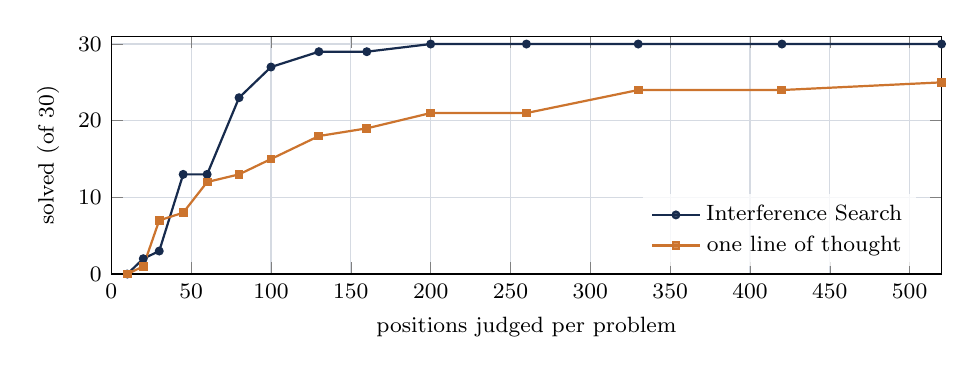
\begin{tikzpicture}
\begin{axis}[width=\columnwidth, height=46mm, xlabel={positions judged per problem}, ylabel={solved (of 30)},
  xmin=0, xmax=520, ymin=0, ymax=31, ytick={0,10,20,30}, grid=major, grid style={btlrule!60},
  legend pos=south east, legend style={font=\footnotesize, draw=none, fill=white, fill opacity=0.8, text opacity=1},
  tick label style={font=\footnotesize}, label style={font=\footnotesize}]
\addplot[btlblue, thick, mark=*, mark size=1.2pt] coordinates {(10,0) (20,2) (30,3) (45,13) (60,13) (80,23) (100,27) (130,29) (160,29) (200,30) (260,30) (330,30) (420,30) (520,30)};
\addlegendentry{\IS}
\addplot[btlamber, thick, mark=square*, mark size=1.2pt] coordinates {(10,0) (20,1) (30,7) (45,8) (60,12) (80,13) (100,15) (130,18) (160,19) (200,21) (260,21) (330,24) (420,24) (520,25)};
\addlegendentry{one line of thought}
\end{axis}
\end{tikzpicture}
\caption{Hard four-number Countdown, same judge and budget for both. The frontier reaches 30 of 30 at 200 judged positions; the line reaches 25 with more than twice that.}
\label{fig:curves}
\end{figure}

Figure~\ref{fig:curves} and Table~\ref{tab:bench} compare the two shapes with the judge held fixed. The frontier solves every problem by 200 judged positions. The line needs 1,500 to solve them all, and then takes 23.7 sequential steps on average against the frontier's 3. Because branches advance together, time follows the depth of the problem rather than the number of mistakes. Wall-clock time on a laptop CPU is a few milliseconds per problem for both (8 to 14 ms for the frontier, 11 to 24 ms for the line) because my implementation executes branches one after another; the step count is what translates into latency when each step is an expensive model call executed in parallel.

\begin{table}[t]
\centering\small
\begin{tabular}{rcccc}
\toprule
 & \multicolumn{2}{c}{One line} & \multicolumn{2}{c}{\IS} \\
\cmidrule(lr){2-3}\cmidrule(lr){4-5}
Budget & Solved & Steps & Solved & Steps \\
\midrule
150 & 19 & 6.8 & 29 & 3.0 \\
200 & 21 & 7.9 & 30 & 3.0 \\
500 & 24 & 10.8 & 30 & 3.0 \\
1,500 & 30 & 23.7 & 30 & 3.0 \\
\bottomrule
\end{tabular}
\caption{Hard four-number problems (30). Steps: mean sequential rounds on solved problems.}
\label{tab:bench}
\end{table}

To locate the gain I compared four arms on 100 unseen six-number problems at matched expansions (Figure~\ref{fig:ablation}). At 100 expansions the merged frontier solves 77\%, the line 40\%, and the frontier without merging 50\%: duplicate states otherwise fill the width, and merging accounts for most of the compute advantage. A global ranked memory of every state seen (best-first search) solves 10\%. It keeps choosing shallow states that look safe and never commits to depth, which is why the frontier's level-synchronous advance matters. The frontier finishes in 5 sequential rounds against the line's 116. On seven-number problems the line catches up at large budgets (87\% for both at 400 expansions); the frontier's advantage is at small and medium budgets.

\begin{figure}[t]
\centering
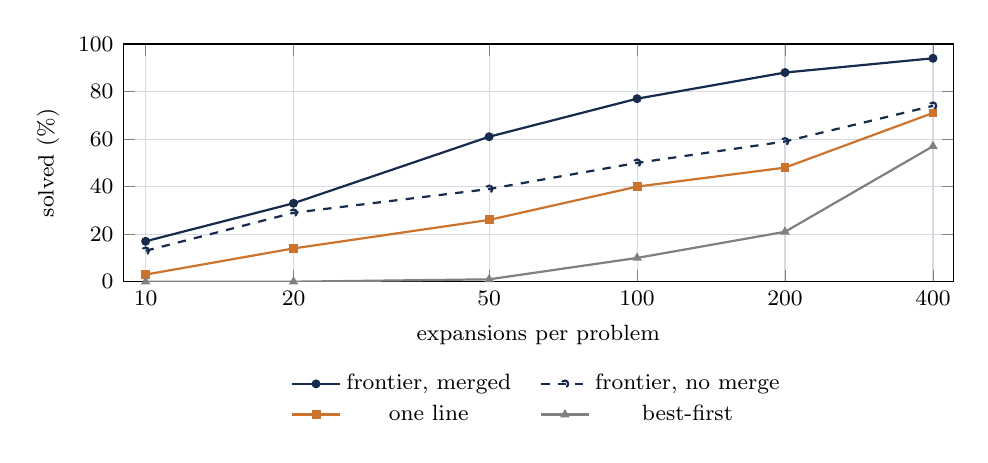
\begin{tikzpicture}
\begin{axis}[width=\columnwidth, height=46mm, xmode=log, log basis x=10, xlabel={expansions per problem}, ylabel={solved (\%)},
  xmin=9, xmax=440, ymin=0, ymax=100, xtick={10,20,50,100,200,400}, xticklabels={10,20,50,100,200,400}, grid=major, grid style={btlrule!60},
  legend style={font=\footnotesize, draw=none, at={(0.5,-0.34)}, anchor=north, legend columns=2, /tikz/every even column/.append style={column sep=3mm}},
  tick label style={font=\footnotesize}, label style={font=\footnotesize}]
\addplot[btlblue, thick, mark=*, mark size=1.2pt] coordinates {(10,17) (20,33) (50,61) (100,77) (200,88) (400,94)};
\addlegendentry{frontier, merged}
\addplot[btlblue, thick, dashed, mark=o, mark size=1.2pt] coordinates {(10,13) (20,29) (50,39) (100,50) (200,59) (400,74)};
\addlegendentry{frontier, no merge}
\addplot[btlamber, thick, mark=square*, mark size=1.2pt] coordinates {(10,3) (20,14) (50,26) (100,40) (200,48) (400,71)};
\addlegendentry{one line}
\addplot[gray, thick, mark=triangle*, mark size=1.2pt] coordinates {(10,0) (20,0) (50,1) (100,10) (200,21) (400,57)};
\addlegendentry{best-first}
\end{axis}
\end{tikzpicture}
\caption{Unseen six-number problems (100), same judge for every arm. Merging carries most of the frontier's advantage; a global best-first memory does worse than a single line.}
\label{fig:ablation}
\end{figure}

A separate experiment asked whether parallel streams discover coordination on their own. In a hidden-goal tree search where every stream sees the same noisy hints, I trained small transformer policies from scratch with grouped policy gradients, with streams either isolated or able to attend to each other. The two tied (0.508 and 0.511 success with four streams), and both stayed below a simple stochastic player with its own memory (0.70) and well below one with shared memory (0.82). Visibility alone did not produce sharing. Coordination had to be an explicit operation, which is what merging and the judge provide.

\section{With a language model}
\label{sec:llm}

On the same 30 hard problems, Qwen3-1.7B with thinking enabled and a 1,500-token budget solves 3. Table~\ref{tab:llm} places it against the search, where the environment lists moves and a judge ranks states.

\begin{table}[t]
\centering\small
\begin{tabularx}{\columnwidth}{Xrr}
\toprule
System & AUC & Solved \\
\midrule
Qwen3-1.7B thinking in text & & 3 \\
\IS, judge = asking the model yes or no & 0.58 & 4 \\
\IS, judge = linear probe on the model's hidden state & 0.87 & 15 \\
\IS, judge = linear probe on number features & 0.94 & 22 \\
\IS, judge = trained set transformer & 0.98 & 23 \\
\bottomrule
\end{tabularx}
\caption{Hard four-number problems (30). AUC: separating alive from dead states on unseen four-number problems. Probes were trained on 1,376 states from 60 other problems; the trained judge on 632,279.}
\label{tab:llm}
\end{table}

Two readings follow. The structure is doing the work: even a probe on crude features, inside the frontier, solves seven times as many problems as the model reasoning alone, in 3 rounds instead of about 1,400 generated tokens. And the model's hidden state carries reachability information that its answer does not (0.87 against 0.58), but no more than simple number features do. I had first read the probe result as the model knowing more than it can say; the feature control does not support that reading.

Three attempts to get this behaviour out of the model without training failed, and each failure is informative. \emph{Textual ledgers:} every 256 tokens, eight streams were told which full expressions they or their siblings had already refuted. Within 80 tokens of a note, 33.6\% of attempts repeated a sibling's refutation, against about 21\% without notes; telling the model an expression is wrong primes it. Solve rates did not change (22, 21 and 22 of 24). \emph{Decode-time rewinding:} when a stream wrote an already-refuted expression it was rewound and resampled; it regenerated the same line up to 16 times, because the cause sits in the context. \emph{State prompting:} showing the model only the current state and asking for a move made it add the first two listed numbers and repeat the same three-step path; with memory and shuffled order it still solved none of a small set.

\section{Code}
\label{sec:code}

In code the proposer has to invent the options. The state is a program together with its behaviour: what it returns or raises on each test. The interpreter is the executor; programs with identical behaviour merge; the judge is the number of tests passed. Each proposal sees only the task, the current program and its test results.

\begin{table}[t]
\centering\small
\begin{tabular}{lr}
\toprule
Strategy (1,500 generated tokens) & Solved \\
\midrule
Agent loop with full chat history & 7 / 30 \\
Revise the latest program & 7 / 30 \\
Fresh attempts (best of $N$) & 8 / 30 \\
\IS & 9 / 30 \\
\bottomrule
\end{tabular}
\caption{MBPP problems \citep{austin2021mbpp} that Qwen3-1.7B fails on its first greedy attempt (30 of 69 such problems among the first 150). A problem counts as solved only within the budget.}
\label{tab:code}
\end{table}

Table~\ref{tab:code} shows parallel strategies ahead of both linear ones, and \IS{} one problem ahead of independent sampling, which is within noise on 30 problems. Behaviour merging removed 83\% of generated programs as duplicates. The agent loop solved nothing after its third round while its history grew. The traces explain the ceiling: when the model's idea is wrong, revisions reproduce it, so search can organize the model's ideas but cannot supply new ones. A stronger proposer or a trained judge is the natural next test.

\section{Related work}

\paragraph{Search over reasoning.} Tree of Thoughts \citep{yao2023tot}, Graph of Thoughts \citep{besta2024got} and RAP \citep{hao2023rap} organize model outputs as search over thoughts; self-consistency \citep{wang2022selfconsistency} samples in parallel and votes over chains of thought \citep{wei2022cot}. FETCH \citep{wang2025fetch} identifies over-exploration of semantically equivalent states as a failure of tree search and merges them by embedding clustering. Transposition tables \citep{zobrist1970} and learned value functions in AlphaZero \citep{silver2018alphazero} are the classical roots of merging and judging.

\paragraph{Parallel reasoning in one model.} APR \citep{pan2025apr} trains spawn and join operations and reports large gains over serial search on Countdown; ThreadWeaver \citep{lian2025threadweaver}, Parallel-R1 \citep{zheng2025parallelr1}, Hogwild! Inference \citep{rodionov2025hogwild} and Multi-Stream LLMs \citep{su2026multistream} let threads run concurrently or see each other. Parallel-Probe \citep{zheng2026probe} and DeepPrune \citep{tu2025deepprune} prune redundant branches from outside. Parason \citep{zhang2026parason} finds that most parallelizable steps in reasoning traces are competing trials. None of these merges the states branches reach or learns to cancel them inside a synchronized frontier.

\paragraph{State instead of transcript.} Atom of Thoughts \citep{teng2025aot}, the Markovian Thinker \citep{aghajohari2025markovian} and PENCIL \citep{yang2025pencil} reduce or bound what a model carries between steps. Continuous thoughts can hold several search frontiers in theory \citep{zhu2025superposition}, though fine-tuned models appear not to use this \citep{rizvi2026illusion}.

\paragraph{Learned search and execution.} Stream of Search \citep{gandhi2024sos} and Searchformer \citep{lehnert2024searchformer} train models on search traces; learned value functions generalize to larger planning problems \citep{aichmuller2026search}. SWE-Search \citep{antoniades2024swesearch} and ParallelEnv \citep{tan2026parallelenv} branch software agents over environment states.

\section{Limitations}

Every result is one seed, and the larger claims rest on 30 problems per condition, 10 in the seven-number test. The strongest Countdown numbers use a small trained judge and an environment that lists moves; they do not run the language model, and the 5 to 14 ms per problem they take is not a speedup of the model itself. The judge exists only for Countdown, where states are exact and labels come from a solver; open domains need learned merge keys and labels from rollouts, which I have not built. In code the gain over independent sampling is within noise. Nothing here trains the language model, so whether a model trained to reason this way keeps these gains is open. Compute is compared in the domain's unit (judged states or generated tokens); prompt tokens and prefill cost differ between arms and are reported in the repository rather than folded in.

\section{Conclusion}

Holding the model and the judge fixed and changing only the shape of the search, from one chain over a transcript to a frontier over merged states, turned 21 solved problems into 30 at equal compute and 24 sequential steps into 3. The gain comes from merging and level-synchronous advance together, and it grows with problem size because the number of paths grows much faster than the number of states. The negative results say where the mechanism must live: prompts and decoding tricks do not produce it in a small model. The next step is to train it into one.

\paragraph{Code and data.} \url{https://github.com/Badtheorylabs/interference-search}, Apache 2.0, with the trained judge, every raw result and the research log.

\balance
\bibliographystyle{plainnat}
{\small \bibliography{references}}

\end{document}
